\documentclass[a4paper,12pt]{article}
\usepackage{fullpage, float, graphicx}
\title{CS26410 Report 3\\
Hide and Seek}
\author{Chris Savill\\\texttt{chs17@aber.ac.uk}}
\begin{document}
\maketitle
\newpage
\tableofcontents
\newpage

\section{Description of algorithms used}

\subsection{Depth-First-Search (DFS) algorithm}
\noindent The DFS algorithm is used to aid in exploring a whole area. The algorithm requires that a stack is used to store the path along which the robot has travelled to get to its current cell on the occupancy grid. The reason it acts as a DFS is because the algorithm keeps the robot searching further rather than restricting it to searching a close area to a start point and then working out.

\begin{figure}[H]
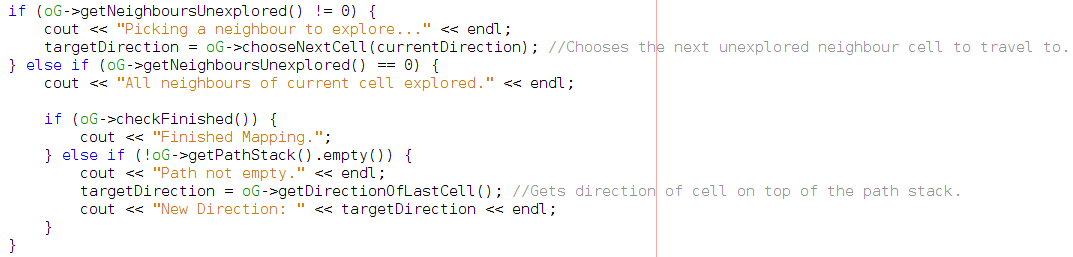
\includegraphics[scale=0.8]{DFS_SS.png}
\caption{Snapshot of DFS code.}
\end{figure}

\vspace{5mm}
\noindent The algorithm has a way of determining if the mapping of an area is complete. The check is a function that evaluates if every cell that has been explored and has no obstacle present, has no unexplored neighbours. If this return true then the search and mapping is complete so the path stack is emptied thus finishing the mapping task.

\begin{figure}[H]
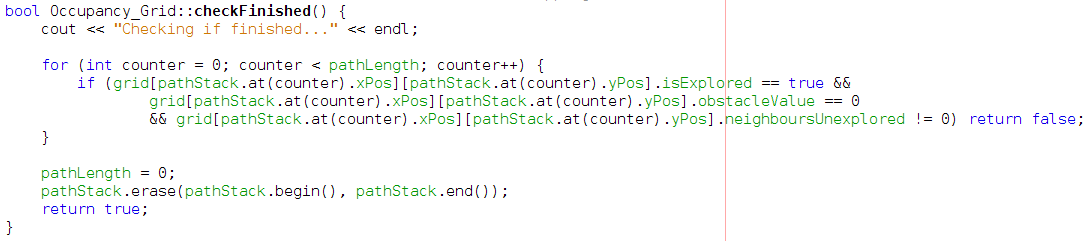
\includegraphics[scale=0.55]{Check_Finished_SS.png}
\caption{Snapshot of check finished function code.}
\end{figure}

\vspace{5mm}
\noindent The way in which the algorithm chooses which direction to continue in at each cell is quite simple. If the cell directly in front of the robot is explorable, the robot will continue in that direction. This was implemented as it speeds up the search because the robot takes a long time to turn. If the cell in front has an obstacle present, a random number is generated that correlates to each of the 4 directions it can travel and checks if that cell is unexplored and has no obstacle present. This random number generator is constantly generated until a cell that is unexplored and is explorable is chosen.

\subsection{Localisation algorithm}
\noindent The localisation algorithm is use to determine whether the robot is within the occupancy grid and if so, where. The algorithm itself works as follows. A new temporary occupancy grid is created for the robot to use for its mapping of its immediate area. Once the immediate area is scanned the temporary grid is compared to all areas of the original occupancy grid. The comparison algorithm uses a 2 for loops to ensure that the temporary grid area is compared to all possible areas of the original grid. The temporary grid is compared to areas of the same size and each individual cell is compared with the corresponding cell of the area being compared with in the original grid.

\begin{figure}[H]
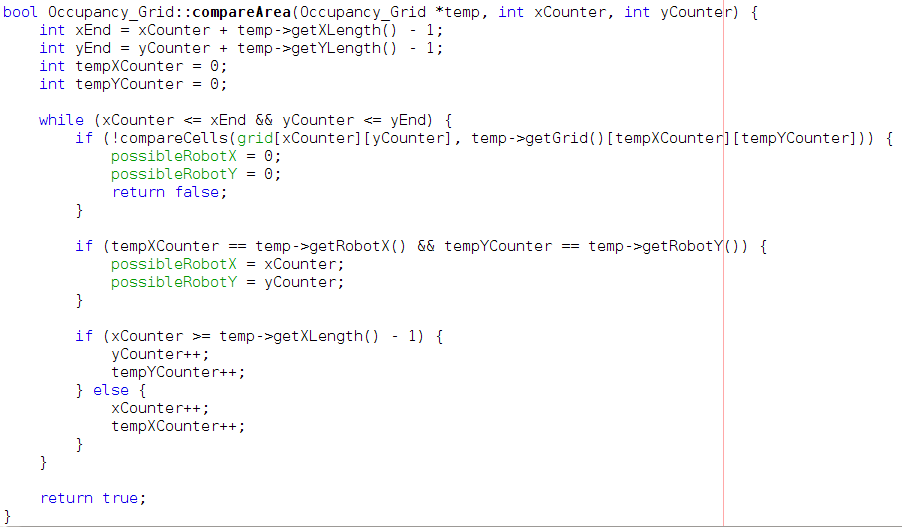
\includegraphics[scale=0.65]{Compare_Area_SS.png}
\caption{Snapshot of compare area function code.}
\end{figure}

\vspace{5mm}
\noindent If the localisation of that area is unsuccessful then the algorithm exits telling the user that the robot is not within the original occupancy grid area. If there is more than 1 place the robot could possible be, the robot uses the DFS algorithm and moves to the next unexplored cell and tries to localise with the additional information gathered. If the comparison algorithm determines that there is only one possible place for the robot to be, the robot switches to using the original occupancy grid and is localised to the area it was found in. As localisation requires that an original occupancy grid exists to compare with, there is a boolean value that tell the robot that it mapped successfully so localisation can be attempted.

\begin{figure}[H]
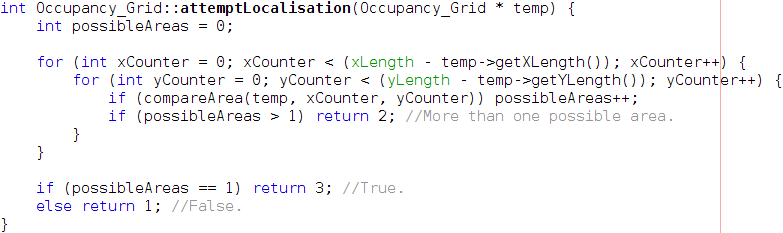
\includegraphics[scale=0.75]{Attempt_Localisation_SS.png}
\caption{Snapshot of attempt localisation function code.}
\end{figure}

\subsection{Hiding algorithm}
\noindent The hiding algorithm consists of 3 parts; the first part involves finding the best place to hide, the second part involves finding the shortest path to that position and the third part involves getting the robot to travel along that path to its hiding location. The hiding function can only be accessed if the localisation of the robot is successful. In order to find the best hiding spot for the robot the algorithm first searches for empty, explored cells and checks if the have 3 walls around them, if none can be found does the same but looks for 2 walls and then 1. 

\begin{figure}[H]
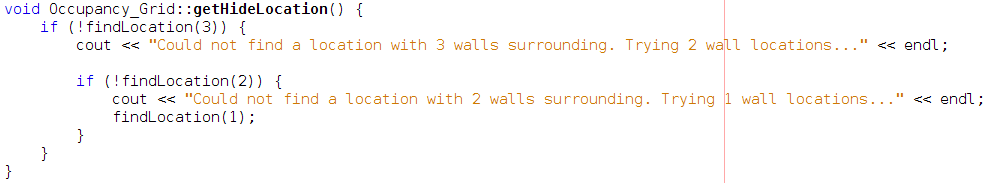
\includegraphics[scale=0.6]{Get_Hide_Location_SS.png}
\caption{Snapshot of code that calls function to search for a hiding place.}
\end{figure}

\begin{figure}[H]
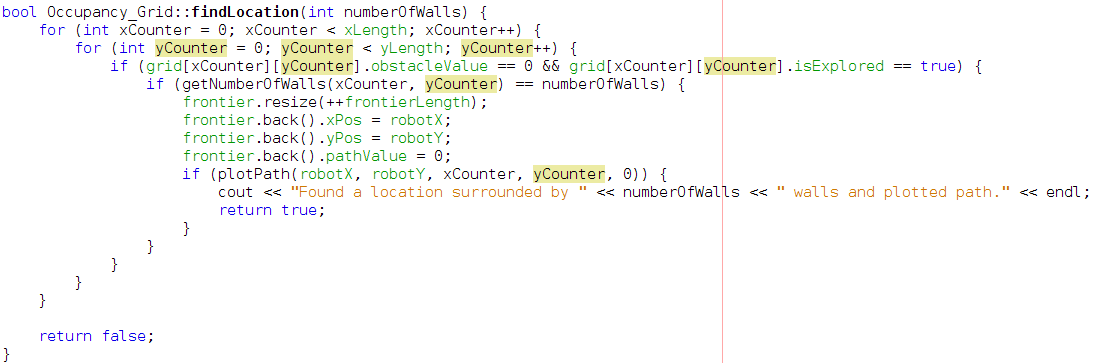
\includegraphics[scale=0.55]{Find_Location_SS.png}
\caption{Snapshot of function that tries to find a hiding location and plot a path using other functions.}
\end{figure}

\vspace{5mm}
\noindent The path finding algorithm is a simple A* search that keeps track of the distance/cost so far and the distance/cost left. The search tries to find the shortest path possible as the search is guided in the direction of the target cell and the total goal value is underestimated not overestimated so it is admissible. Once the path as been plotted from the robot's current location to its hiding location, the robot moves cell by cell along its path until the path stack is empty, at which point the robot should be at its hiding location.

\begin{figure}[H]
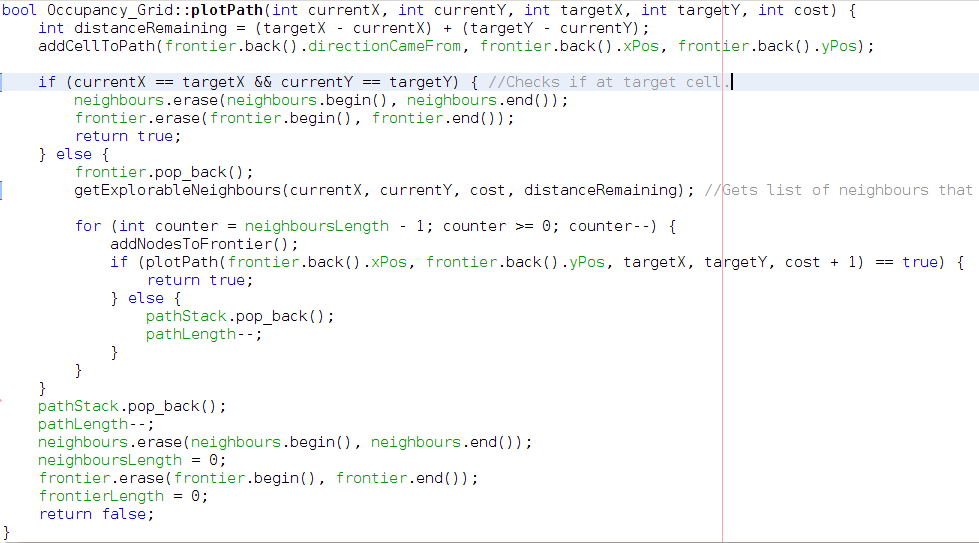
\includegraphics[scale=0.6]{Plot_Path_SS.png}
\caption{Snapshot of function that uses performs an A* search with the aid of other functions.}
\end{figure}

\subsection{Seeking algorithm}
\noindent The seeking algorithm is very simple, if the robot localised successfully, the robot will perform a DFS of the whole pre-explored area, if however any cells that did not contain an obstacle on the original occupancy grid are detected to have an obstacle, then the DFS finishes and the anomaly is stated to the user, thus finishing the seeking function.

\begin{figure}[H]
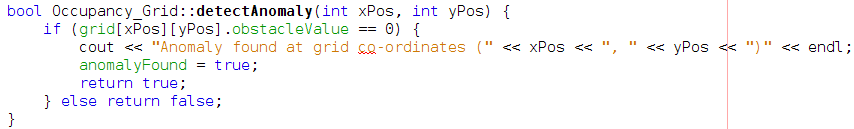
\includegraphics[scale=0.65]{Detect_Anomaly_SS.png}
\caption{Snapshot of function that determines if an anomaly has been found.}
\end{figure}

\section{Trial runs}

\subsection{Simulated trial runs}
\noindent In order to perform real world trials, the robot program first had to be tested through the use of Player/Stage. Before testing proceeding onto real world trials, the robot had to successfully map the whole area of the simulated world provided. Many of the runs were unsuccessful resulting in the robot crashing at some point. Below is a series of screen shots of one of the successful trials for mapping:

\vspace{5mm}
\noindent Key:
\begin{itemize}
\item \# = Obstacle present
\item \textasciitilde = Unexplored cell
\item R = Robot's current location
\item An empty cell represents an explored cell with no obstacle present.
\end{itemize}

\begin{figure}[H]
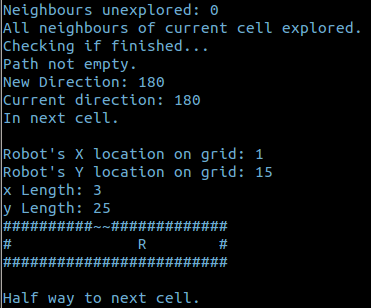
\includegraphics[scale=1.0]{RunT1.png}
\caption{Screen shot of the terminal window corresponding to the screen shot below. Having mapped the the bottom area and hitting a dead end, the robot return along its path to the next available unexplored cell.}
\end{figure}

\begin{figure}[H]
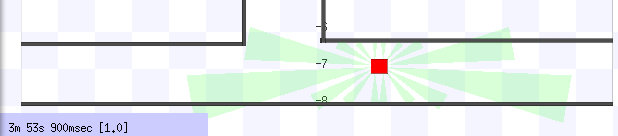
\includegraphics[scale=0.9]{RunS1.png}
\caption{Screen shot of the Stage window corresponding to the screen shot above.}
\end{figure}

\begin{figure}[H]
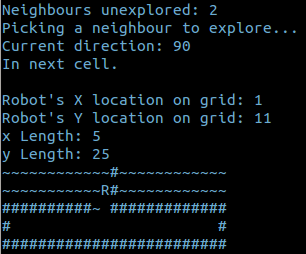
\includegraphics[scale=1.0]{RunT2.png}
\caption{Screen shot of the terminal window corresponding to the screen shot below. Having found the next unexplored cell the robot starts to travel and map upwards.}
\end{figure}

\begin{figure}[H]
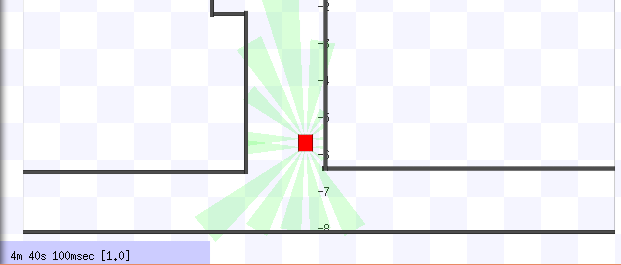
\includegraphics[scale=0.9]{RunS2.png}
\caption{Screen shot of the Stage window corresponding to the screen shot above.}
\end{figure}

\begin{figure}[H]
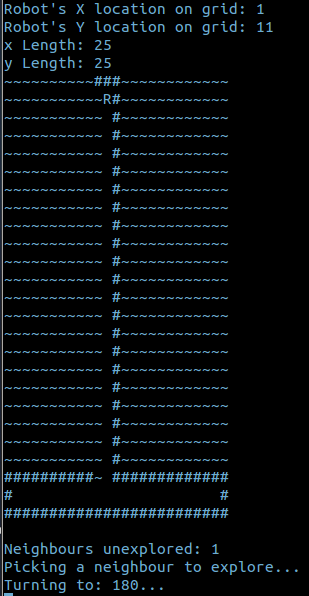
\includegraphics[scale=1.0]{RunT3.png}
\caption{Screen shot of the terminal window corresponding to the screen shot below. Having reached the top the robot turns left as it is the only neighbour cell unexplored.}
\end{figure}

\begin{figure}[H]
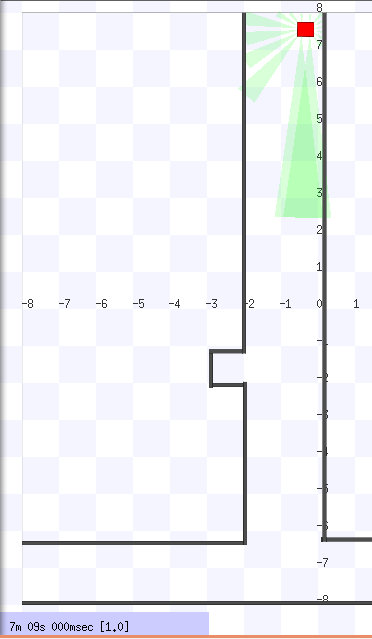
\includegraphics[scale=0.9]{RunS3.png}
\caption{Screen shot of the Stage window corresponding to the screen shot above.}
\end{figure}

\begin{figure}[H]
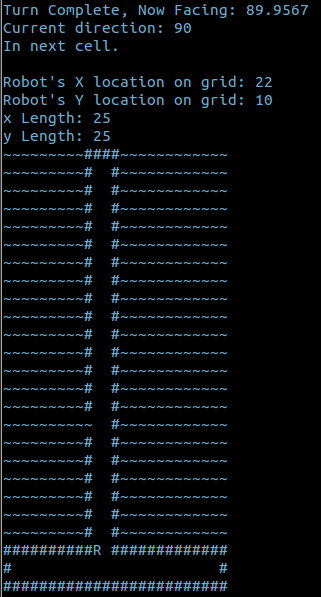
\includegraphics[scale=1.0]{RunT4.png}
\caption{Screen shot of the terminal window corresponding to the screen shot below. Having scanned the left side all the way back to the pre-explored area, the robot turns to travel back along its path to the next unexplored cell.}
\end{figure}

\begin{figure}[H]
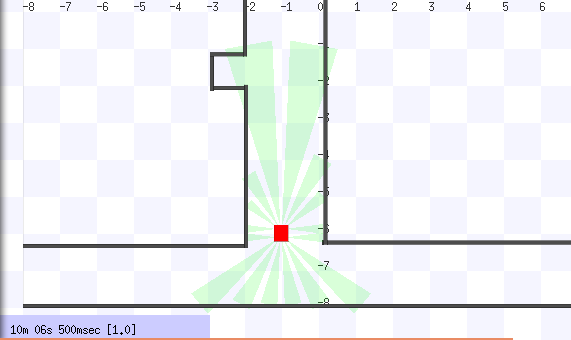
\includegraphics[scale=0.9]{RunS4.png}
\caption{Screen shot of the Stage window corresponding to the screen shot above.}
\end{figure}

\begin{figure}[H]
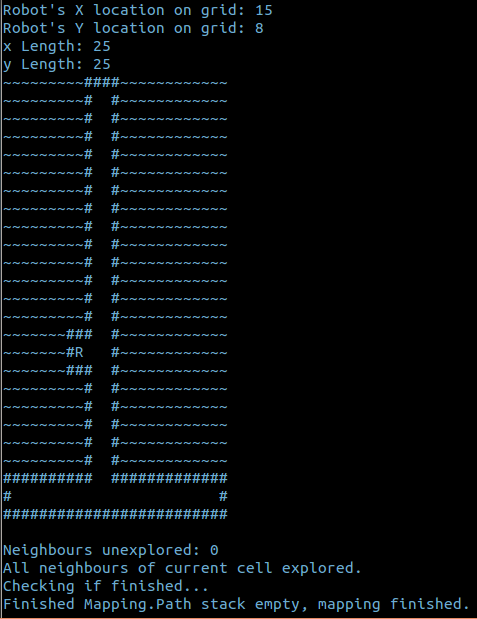
\includegraphics[scale=1.0]{RunT5.png}
\caption{Screen shot of the terminal window corresponding to the screen shot below. Having reached a dead end, the robot evaluates if it has any cells left to explore. As it evaluates there are none, the mapping is declared finished.}
\end{figure}

\begin{figure}[H]
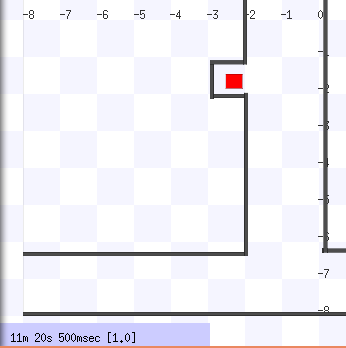
\includegraphics[scale=0.9]{RunS5.png}
\caption{Screen shot of the Stage window corresponding to the screen shot above.}
\end{figure}
\subsection{Real world trial runs}

\section{Discussion of trial run results}

\section{Evaluation of work done}

\subsection{Positive parts}

\subsection{Negative parts}

\subsection{Hardest parts}

\subsection{What would be done differently}
\end{document}